\documentclass[
    article,
    sumario=tradicional,
	% -- opções da classe memoir --
	12pt,				% tamanho da fonte
	openright,			% capítulos começam em pág ímpar (insere página vazia caso preciso)
	oneside,			% para impressão em verso e anverso. Oposto a oneside
	a4paper,			% tamanho do papel. 
	% -- opções da classe abntex2 --
	%chapter=TITLE,		% títulos de capítulos convertidos em letras maiúsculas
	section=TITLE,		% títulos de seções convertidos em letras maiúsculas
	%subsection=TITLE,	% títulos de subseções convertidos em letras maiúsculas
	%subsubsection=TITLE,% títulos de subsubseções convertidos em letras maiúsculas
	% -- opções do pacote babel --
	%english,			% idioma adicional para hifenização
	%french,				% idioma adicional para hifenização
	%spanish,			% idioma adicional para hifenização
	brazil				% o último idioma é o principal do documento
	]{abntex2}

\usepackage{ifthen,ifpdf}

\ifpdf
  \pdfpagewidth=\paperwidth
  \pdfpageheight=\paperheight
\fi

% --- 
% CONFIGURAÇÕES DE PACOTES
% --- 
% ---
% Pacotes básicos 
% ---
\usepackage{lmodern}			% Usa a fonte Latin Modern			
\usepackage[T1]{fontenc}		% Selecao de codigos de fonte.
\usepackage[utf8]{inputenc}		% Codificacao do documento (conversão automática dos acentos)
\usepackage{lastpage}			% Usado pela Ficha catalográfica
\usepackage{indentfirst}		% Indenta o primeiro parágrafo de cada seção.
\usepackage{color}				% Controle das cores
\usepackage{graphicx}			% Inclusão de gráficos
\usepackage{microtype} 			% para melhorias de justificação
\usepackage{ufc-abntex2}
\usepackage{enumitem}
\usepackage{amsmath}
\usepackage{booktabs}
\usepackage{multirow}
\usepackage{titlesec}
\usepackage{mathptmx}                               % Usa a fonte Times New Roman
\usepackage{float}
%formatação do Sumário
\usepackage{etoolbox}                               
% Usado para alterar a fonte da Section no Sumário
\usepackage[nogroupskip,nonumberlist,acronym]{glossaries}                %
% ---
		
% ---
% Pacotes adicionais, usados apenas no âmbito do Modelo Canônico do abnteX2
% ---
\usepackage{lipsum}				% para geração de dummy text
% ---

% ---
% Pacotes de citações
% ---
%\usepackage[brazilian,hyperpageref]{backref}	 % Paginas com as citações na bibl
%\usepackage[alf]{abntex2cite}	% Citações padrão ABNT

%Com et al nas referências
%\usepackage[alf, abnt-emphasize=bf, bibjustif, recuo=0cm, abnt-etal-cite=3, abnt-etal-text=it, abnt-etal-list=3]{abntex2cite} 

%Sem et al nas referências
\usepackage[alf, abnt-emphasize=bf, bibjustif, recuo=0cm, abnt-etal-cite=3, abnt-etal-text=it, abnt-etal-list=0]{abntex2cite} 

% Ambiente para alineas e e subalineas (incisos) com ponto
\newlist{alineascomponto}{itemize}{2}
\setlist[alineascomponto,1]{label={$\bullet$},topsep=0pt,itemsep=0pt,leftmargin=\parindent+\labelwidth-\labelsep}%
\setlist[alineascomponto,2]{label={--},topsep=0pt,itemsep=0pt,leftmargin=*}
\newlist{subalineascomponto}{enumerate}{1}
\setlist[subalineascomponto,1]{label={$\circ$},topsep=0pt,itemsep=0pt,leftmargin=*}%
% ---

% Ambiente para alineas e e subalineas (incisos) com numeros
\newlist{alineascomnumero}{enumerate}{2}
\setlist[alineascomnumero,1]{label={$\arabic*$.},topsep=0pt,itemsep=0pt,leftmargin=\parindent+\labelwidth-\labelsep}%
\setlist[alineascomnumero,2]{label={--},topsep=0pt,itemsep=0pt,leftmargin=*}
\newlist{subalineascomnumero}{enumerate}{1}
\setlist[subalineascomnumero,1]{label={$\arabic*$.},topsep=0pt,itemsep=0pt,leftmargin=*}%
% ---

% ---
% Configurações do pacote backref
% Usado sem a opção hyperpageref de backref
%\renewcommand{\backrefpagesname}{Citado na(s) página(s):~}
% Texto padrão antes do número das páginas
%\renewcommand{\backref}{}
% Define os textos da citação
%\renewcommand*{\backrefalt}[4]{
%	\ifcase #1 %
%		Nenhuma citação no texto.%
%	\or
%		Citado na página #2.%
%	\else
%		Citado #1 vezes nas páginas #2.%
%	\fi}%
% ---

% ---
% Configurações de aparência do PDF final

% alterando o aspecto da cor azul
\definecolor{blue}{RGB}{41,5,195}

% informações do PDF
\makeatletter
\hypersetup{
     	%pagebackref=true,
		pdftitle={\@title}, 
		pdfauthor={\@author},
    	pdfsubject={\imprimirpreambulo},
	    pdfcreator={LaTeX with abnTeX2},
		pdfkeywords={abnt}{latex}{abntex}{abntex2}{trabalho acadêmico}, 
		colorlinks=true,       		% false: boxed links; true: colored links
    	linkcolor=blue,          	% color of internal links
    	citecolor=blue,        		% color of links to bibliography
    	filecolor=magenta,      		% color of file links
		urlcolor=blue,
		bookmarksdepth=4
}
\makeatother
% --- 

\makeatletter
\def\@biblabel#1{}
\renewenvironment{thebibliography}[1]
     {\section*{\refname}%
      \@mkboth{\MakeUppercase\refname}{\MakeUppercase\refname}%
      \list{\@biblabel{\@arabic\c@enumiv}}%
           {\settowidth\labelwidth{\@biblabel{#1}}%
            \leftmargin\labelwidth
            %\advance\leftmargin\labelsep
            \@openbib@code
            \usecounter{enumiv}%
            \let\p@enumiv\@empty
            \renewcommand\theenumiv{\@arabic\c@enumiv}}%
      \sloppy
      \clubpenalty4000
      \@clubpenalty \clubpenalty
      \widowpenalty4000%
      \sfcode`\.\@m}
     {\def\@noitemerr
       {\@latex@warning{Empty `thebibliography' environment}}%
      \endlist}
\makeatother

% --- 
% Espaçamentos entre linhas e parágrafos 
% --- 

% O tamanho do parágrafo é dado por:
\setlength{\parindent}{1.5cm}


\setlength{\parindent}{2cm}

% ---
% compila o indice
% ---
\makeindex
% ---


% Define as margens do documento
\setlrmarginsandblock{3cm}{2cm}{*} % externa / interna
\setulmarginsandblock{3cm}{2cm}{*} % superior / inferior

% Define o espaço entre linhas para 1.5 cm
%\OnehalfSpacing	Bug no ABNTEX2?
\renewcommand{\baselinestretch}{1.5}



\usepackage{hyperref}% http://ctan.org/pkg/hyperref
\hypersetup{%
  colorlinks = false,
  linkcolor  = black
}

% Informações de dados para CAPA e FOLHA DE ROSTO
\titulo{TÍTULO TÍTULO TÍTULO TÍTULO  TÍTULO TÍTULO TÍTULO TÍTULO TÍTULO TÍTULO TÍTULO TÍTULO TÍTULO TÍTULO }
\autor{Nome Autor}
\local{Quixadá}
\data{Abril, 2016}
\orientador{Nome Orientador}
\coorientador{Nome Coorientador}

% Escolher curso: Redes de Computadores (rc), Eng.Software (es), Ciências da Computação (cc) ou Sist.Informação (si)
%\instituicao{%
Universidade Federal do Ceará \par
Campus Quixadá \par
Curso de Redes de Computadores
}

\ies{Universidade Federal do Ceará}
\campus{Campus de Quixadá}
\curso{Curso de Redes de Computadores}

\tipotrabalho{Trabalho de Conclusão de Curso (Monografia)}
\preambulo{Monografia apresentada ao Curso de Redes de Computadores do Campus Quixadá da Universidade Federal do Ceará, como requisito parcial para obtenção do Título de Tecnólogo em Redes de Computadores.}

%\instituicao{%
Universidade Federal do Ceará \par
Campus Quixadá \par
Curso de Sistemas de Informação
}

\ies{Universidade Federal do Ceará}
\campus{Campus de Quixadá}
\curso{Curso de Sistemas de Informação}

\tipotrabalho{Trabalho de Conclusão de Curso (Monografia)}
\preambulo{Monografia apresentada ao Curso de Sistemas de Informação do Campus Quixadá da Universidade Federal do Ceará, como requisito parcial para obtenção do Título de Bacharel em Sistemas de Informação.}

\instituicao{
Universidade Federal do Ceará \par
Campus de Quixadá \par
Curso de Engenharia de Software
}

\ies{Universidade Federal do Ceará}
\campus{Campus de Quixadá}
\curso{Curso de Engenharia de Software}

\tipotrabalho{Trabalho de Conclusão de Curso (Monografia)}
\preambulo{Monografia apresentada ao Curso de Engenharia de Software do Campus Quixadá da Universidade Federal do Ceará, como requisito parcial para obtenção do Título de Bacharel em Engenharia de Software.}

%\instituicao{%
Universidade Federal do Ceará \par
Campus Quixadá \par
Curso de Ciência da Computação
}


\ies{Universidade Federal do Ceará}
\campus{Campus de Quixadá}
\curso{Curso de Ciência da Computação}

\tipotrabalho{Trabalho de Conclusão de Curso (Monografia)}
\preambulo{Monografia apresentada ao Curso de Ciências da Computação do Campus Quixadá da Universidade Federal do Ceará, como requisito parcial para obtenção do Título de Bacharel em Ciências da Computação.}
 

%%criar um novo estilo de cabeçalhos e rodapés
\makepagestyle{header_style}
  %%cabeçalhos
  \makeoddhead{header_style} %%pagina ímpar ou com oneside
     {}
     {}
     {\thepage} 


\begin{document}
\frenchspacing 

%Formatação de título de seções
\titleformat{\section}
{\normalfont\normalsize\bfseries}{\thesection}{1em}{}
\titleformat{\subsection}
{\normalfont\normalsize\bfseries}{\thesubsection}{1em}{}
\titleformat{\subsubsection}
{\normalfont\normalsize\bfseries}{\thesubsubsection}{1em}{}

\renewcommand{\cftsectionfont}{\normalfont\normalsize}   
\renewcommand{\cftsubsectionfont}{\normalfont\normalsize} 
\renewcommand{\cftsubsubsectionfont}{\normalfont\normalsize}  

% ----------------------------------------------------------
% ELEMENTOS PRÉ-TEXTUAIS
% ----------------------------------------------------------
% \pretextual
% Capa
\imprimircapa

%----------- Apenas TCC 2
% Folha de rosto (* indica que haverá a ficha bibliográfica)
%\imprimirfolhaderosto

% Ficha Bibliográfica
%% ---
% Inserir a ficha bibliografica
% ---

% Isto é um exemplo de Ficha Catalográfica, ou ``Dados internacionais de
% catalogação-na-publicação''. Você pode utilizar este modelo como referência. 
% Porém, provavelmente a biblioteca da sua universidade lhe fornecerá um PDF
% com a ficha catalográfica definitiva após a defesa do trabalho. Quando estiver
% com o documento, salve-o como PDF no diretório do seu projeto e substitua todo
% o conteúdo de implementação deste arquivo pelo comando abaixo:
%
% \begin{fichacatalografica}
%     \includepdf{fig_ficha_catalografica.pdf}
% \end{fichacatalografica}
\begin{fichacatalografica}
	\vspace*{\fill}					% Posição vertical
	\hrule							% Linha horizontal
	\begin{center}					% Minipage Centralizado
	\begin{minipage}[c]{12.5cm}		% Largura
	
	\imprimirautor
	
	\hspace{0.5cm} \imprimirtitulo  / \imprimirautor. --
	\imprimirlocal, \imprimirdata-
	
	\hspace{0.5cm} \pageref{LastPage} p. : il. (algumas color.) ; 30 cm.\\
	
	\hspace{0.5cm} \imprimirorientadorRotulo~\imprimirorientador\\
	
	\hspace{0.5cm}
	\parbox[t]{\textwidth}{\imprimirtipotrabalho~--~\imprimirinstituicao,
	\imprimirdata.}\\
	
	\hspace{0.5cm}
		1. Palavra-chave1.
		2. Palavra-chave2.
		I. Orientador.
		II. Universidade xxx.
		III. Faculdade de xxx.
		IV. Título\\ 			
	
	\hspace{8.75cm} CDU 02:141:005.7\\
	
	\end{minipage}
	\end{center}
	\hrule
\end{fichacatalografica}
% ---

% Errata
%% ---
% Inserir errata
% ---
\begin{errata}
Elemento opcional da NORMA. Exemplo:

\vspace{\onelineskip}

FERRIGNO, C. R. A. \textbf{Tratamento de neoplasias ósseas apendiculares com
reimplantação de enxerto ósseo autólogo autoclavado associado ao plasma
rico em plaquetas}: estudo crítico na cirurgia de preservação de membro em
cães. 2011. 128 f. Tese (Livre-Docência) - Faculdade de Medicina Veterinária e
Zootecnia, Universidade de São Paulo, São Paulo, 2011.

\begin{table}[htb]
\center
\footnotesize
\begin{tabular}{|p{1.4cm}|p{1cm}|p{3cm}|p{3cm}|}
  \hline
   \textbf{Folha} & \textbf{Linha}  & \textbf{Onde se lê}  & \textbf{Leia-se}  \\
    \hline
    1 & 10 & auto-conclavo & autoconclavo\\
   \hline
\end{tabular}
\end{table}

\end{errata}
% ---


% Folha de Aprovação
% DEVE ser modificada para adicionar os membros da banca
%% ---
% Inserir folha de aprovação
% ---

% Isto é um exemplo de Folha de aprovação, elemento obrigatório da NBR
% 14724/2011 (seção 4.2.1.3). Você pode utilizar este modelo até a aprovação
% do trabalho. Após isso, substitua todo o conteúdo deste arquivo por uma
% imagem da página assinada pela banca com o comando abaixo:
%
% \includepdf{folhadeaprovacao_final.pdf}
%
\begin{folhadeaprovacao}

  \begin{center}
    {\bfseries\Large\imprimirautor}
    \vspace{1cm}

    \begin{center}
      \bfseries\Large\imprimirtitulo
    \end{center}

    \vspace{2cm}
    \begin{minipage}{\textwidth}
        \imprimirpreambulo
        \\ \\ \\
        Aprovada em: \_\_/\_\_/\_\_\_\_
    \end{minipage}%
     
    \vspace{2cm}
	\textbf{BANCA EXAMINADORA}
   \end{center}
	

   \assinatura{\imprimirorientador \space (Orientador) \\ Universidade Federal do Ceará (UFC)}
   \assinatura{\imprimircoorientador \space Rossana Maria de Castro Andrade \\ Universidade Federal do Ceará (UFC)}
   %DEFINA AQUI OS DEMAIS MEMBROS DA BANCA
   \assinatura{Márcio Espíndola Freire Maia \\ Universidade Federal do Ceará (UFC)}
   %\assinatura{Prof. Dr. Alguma Coisa \\ Instituição}
   %\assinatura{Prof. Msc. Alguma Coisa \\ Instituição}
      
%   \begin{center}
%    \vspace*{0.5cm}
%    {\large\imprimirlocal}
%    \par
%    {\large\imprimirdata}
%    \vspace*{1cm}
%  \end{center}
  
\end{folhadeaprovacao}
% ---

%\imprimirfolhadeaprovacao

% Dedicatória
%% ---
% Dedicatória
% ---
\begin{dedicatoria}
   \vspace*{\fill}
   	\begin{flushright}
   \noindent
    Este trabalho é dedicado a um pai, a uma mãe e a uma irmã esperançosa, que acreditou neste sonho que se tornou realidade.
   	\end{flushright}
\end{dedicatoria}
% ---

% Agradecimentos
%% ---
% Agradecimentos
% ---
\begin{agradecimentos}
	Os agradecimentos principais são direcionados à Antônia da Silva Pinho, Carlos Luís Pinho, João Filho Costa, Etinha Lima e a todos que acrescentaram sua inestimável contribuição à minha formação pessoal e acadêmica.

	Agradecimentos especiais são direcionados aos professores que fazem parte da minha história, principalmente à primeira de todas, minha irmã Lúcia Braz.
\end{agradecimentos}
% ---

% Epígrafe
%% ---
% Epígrafe
% ---
\begin{epigrafe}
    \vspace*{\fill}
	\begin{flushright}
		\textit{``Pode se encontrar a felicidade mesmo nas horas mais sombrias, se a pessoa se lembrar de acender a luz.``\\
		(J. K. Rowling)}
	\end{flushright}
\end{epigrafe}
% ---

% RESUMOS
%% resumo em português
\setlength{\absparsep}{18pt} % ajusta o espaçamento dos parágrafos do resumo
\begin{resumo}
 Segundo a NBR6028:2003, o resumo deve ressaltar o
 objetivo, o método, os resultados e as conclusões do documento. A ordem e a extensão
 destes itens dependem do tipo de resumo (informativo ou indicativo) e do
 tratamento que cada item recebe no documento original. O resumo deve ser
 precedido da referência do documento, com exceção do resumo inserido no
 próprio documento. (\ldots) As palavras-chave devem figurar logo abaixo do
 resumo, antecedidas da expressão Palavras-chave:, separadas entre si por
 ponto e finalizadas também por ponto.

 \textbf{Palavras-chaves}: latex. abntex. editoração de texto.
\end{resumo}
%% resumo em inglês
\begin{resumo}[Abstract]
 \begin{otherlanguage*}{english}
   This is the english abstract.

   \vspace{\onelineskip}
 
   \noindent 
   \textbf{Key-words}: latex. abntex. text editoration.
 \end{otherlanguage*}
\end{resumo}
%% resumo em francês 
\begin{resumo}[Résumé]
 \begin{otherlanguage*}{french}
    Il s'agit d'un résumé en français.
 
   \textbf{Mots-clés}: latex. abntex. publication de textes.
 \end{otherlanguage*}
\end{resumo}

%% resumo em espanhol
\begin{resumo}[Resumen]
 \begin{otherlanguage*}{spanish}
   Este es el resumen en español.
  
   \textbf{Palabras clave}: latex. abntex. publicación de textos.
 \end{otherlanguage*}
\end{resumo}
% ---

% Lista de ilustrações
%\pdfbookmark[0]{\listfigurename}{lof}
%\listoffigures*
%\clearpage

% Lista de tabelas
%\pdfbookmark[0]{\listtablename}{lot}
%\listoftables*
%\cleardoublepage

% Abreviaturas e Siglas
%% Lista de abreviaturas e siglas
% ---
\begin{siglas}
  \item[ABNT] Associação Brasileira de Normas Técnicas
  \item[abnTeX] ABsurdas Normas para TeX
\end{siglas}
% ---

% Símbolos
%%Lista de símbolos
% ---
\begin{simbolos}
  \item[$ \Gamma $] Letra grega Gama
  \item[$ \Lambda $] Lambda
  \item[$ \zeta $] Letra grega minúscula zeta
  \item[$ \in $] Pertence
\end{simbolos}
% ---
%----------- fim - Apenas TCC 2


% Sumário

\imprimirsumario

% ----------------------------------------------------------
% ELEMENTOS TEXTUAIS
% ----------------------------------------------------------
\textual

%aplicação de estilo de cabeçalho
\pagestyle{header_style}

%uso do input pois o include dá quebra de página no final
\section{INTRODUÇÃO}

% --- Espaço aéreo geral
A Administração Federal de Aviação dos Estados Unidos (FAA) está evoluindo para a próxima geração de sistemas de transporte aéreo com uma atualização completa de seus sistemas e tecnologias visando reduzir os atrasos, economizar combustível, diminuir a emissão de carbono e aumentar a segurança dos voos. Essa iniciativa integra novas e existentes tecnologias, incluindo a navegação por satélite e comunicações digitais avançadas \cite{faa2015}.

Essa necessidade de ampla atualização surge por ainda se operar mundialmente com vários sistemas e técnicas de monitoramento aéreo ultrapassados. As atuais tecnologias para evitar colisões entre aeronaves, estão se tornando inadequadas. O sistema mais comum para esse fim, Traffic Alert and Collision Avoidance System (TCAS), já é bastante antigo e não é capaz de acompanhar as métricas previstas para a nova geração de sistemas. É necessário, como sujere \citeonline{Chamlou2008}, que algumas tecnologias sejam revistas e novas soluções sejam adotadas.

O sistema TCAS funciona dentro das aeronaves, alertando os pilotos sobre possíveis conflitos com as aeronaves vizinhas. O TCAS I, primeira geração da tecnologia anunciada em 1981, monitora o tráfego ao redor da aeronave em um raio de 65 km e oferece informações de direção e altitude de outras aeronaves. Esta versão oferece ao piloto alertas de colisão na forma Traffic Advisory (TA), que emite um alerta sonoro sobre a proximidade de outra aeronave. Cabe ao piloto a resolução do conflito. O TCAS II foi introduzido em 1989 e é usado na maioria dos equipamentos da aviação comercial atual. O sistema opera de forma sincronizada entre as aeronaves, gerando alertas do tipo Resolution Advisory (RA) fornecendo sugestões de mudança de rota aos pilotos para evitar colisões. O sistema TCAS III foi concebido como uma extensão do sistema TCAS II, permitindo aos pilotos manobras horizontais, além das verticais presentes nas outras versões. Porém, a antena direcional utilizada no posicionamento vertical da aeronave não era precisa o suficiente, e o TCAS IV substituiu o TCAS III em meados de 1990, utilizando informações adicionais de posicionamento global para gerar uma resolução horizontal mais precisa. O desenvolvimento TCAS IV continuou por alguns anos, mas foi abandonado com o surgimento de novas tecnologias, tais como a Automatic Dependent Surveillance-Broadcast (ADS-B), uma tecnologia moderna e acessível desenvolvida para auxiliar o atual sistema baseado em radares no monitoramento de aeronaves civis \cite{Williamson1989}.

% --- Problemática colisão

Colisões entre aeronaves são um grande problema para os sistemas de monitoramento aéreo. Segundo o Escritório de Registros de Acidentes Aéreos\footnote{http://www.baaa-acro.com} (ACRO), no período de 1918 até 2016 foram registrados 23.670 acidentes aéreos com 146.726 mortes, dos quais 7.625 foram causados por falha humana. Isso tende a se agravar com o aumento do tráfego de aeronaves de pequeno porte, Very Light Aircrafts (VLA), pertencentes a empresas pequenas e que operam em aeroportos secundários. Um tráfego aéreo mais denso traz a necessidade de sistemas e algoritmos mais robustos, que possam gerenciar muitas aeronaves simultaneamente.

Os algoritmos computacionais mais comuns para esse propósito, como esclarece \citeonline{Carbone2006}, são formulados como problemas de otimização e a convergência para uma solução não é garantida em um intervalo de tempo finito e determinístico. Assim, ainda segundo \citeonline{Carbone2006}, o algoritmo se comporta de formas diferentes para uma mesma situação de entrada de dados e não é possível prever seu tempo de execução, comportamento exigido por um sistema de controle aéreo em tempo real.

% --- Problemática no contexto do espaço aéreo
No Brasil a problemática é semelhante. Sistemas antigos ainda operam no país, embora já existam alternativas mais baratas e confiáveis. Grande parte do nosso sistema de monitoramento aéreo ainda é baseado em radares. Assim, a eficiência do monitoramento é sujeita a falhas e a prevenção contra colisão de aeronaves é potencialmente problemática. 

% --- Problemática no contexto do Radar Livre
    % --- Solução ADS-B
Para auxiliar o sistema aéreo brasileiro a acompanhar os avanços tecnológicos da FAA, um grupo de pesquisa da Universidade Federal do Ceará (UFC) em Quixadá está desenvolvendo o Sistema de Monitoramento do Espaço Aéreo Radar Livre, uma solução mista de hardware e software baseada na tecnologia Automatic Dependent Surveillance-Broadcast (ADS-B) que proporciona uma base de dados centralizada com todos os dados coletados e uma interface de monitoramento onde as informações podem ser visualizadas graficamente. O sistema opera fora das aeronaves, em um servidor Web, sendo mais adequado ao uso de controladores de voo, e já conta com alguns de seus módulos em funcionamento, como a coleta de dados de aeronaves, um banco de dados online com as informações coletadas e um site, onde as mesmas podem ser acessadas\footnote{Ressalta-se que o sistema possui coletores em funcionamento apenas no estado do Ceará, os quais capturam dados de uma pequena quantidade de aeronaves diariamente. O site do sistema Radar Livre disponibiliza publicamente todas as informações coletadas, e está disponível em www.radarlivre.com}. Dentre suas atuais propostas, destaca-se o desenvolvimento de um módulo de previsão de colisão entre aeronaves e entre aeronaves e acidentes geográficos. 

% --- Explicação do motivo do trabalho nos contextos anteriores

    % --- O trabalho nasce do projeto Radar Livre
    % --- O que o trabalho promete
    % --- Resultados "pretendidos" 

Em aeroportos é comum a utilização de aves de rapina na prevenção contra conflitos entre aves e aeronaves. Por seu objetivo igualmente nobre, o módulo de detecção de colisão do sistema Radar Livre recebeu o apelido de CAPLAN, contração de \textit{Caracara Plancus}, nome científico de uma ave de rapina comum no estado do Ceará. Além de um algoritmo de detecção de colisão eficaz e eficiente, o CAPLAN necessita de alternativas para lidar com milhares de aeronaves simultaneamente. Com foco apenas na detecção de colisões entre aeronaves, o presente trabalho nasce com o intuito de propor e avaliar o desempenho de uma solução para aplicação em grande escala de um algoritmo de detecção de colisão entre aeronaves no espaço aéreo, o qual fará parte do futuro sistema de previsão de colisão do sistema de monitoramento Radar Livre.


\section{TRABALHOS RELACIONADOS}

Em seu trabalho, \citeonline{Carbone2006} apresentam um algoritmo para detecção e tratamento de colisões utilizando-se de geometria tridimensional. O mesmo é apresentado como uma alternativa aos algoritmos existentes até então, que não operavam rápido o suficiente. No método, as aeronaves são tratadas como vetores tridimensionais. Uma das aeronaves, considerada como um referencial, é o centro de uma esfera que define um volume de segurança em torno da mesma. Se uma outra aeronave cruzar essa fronteira, estará na iminência de uma colisão. Por ser simples e direto, o algoritmo pode ser executado rapidamente adequando-se a aplicações de tempo real. O método não considera, no entanto, possíveis variantes na orientação e velocidades das aeronaves, o que o torna pouco preciso.

\citeonline{Gariel2011} apresentam uma solução que considera variantes de orientação e velocidade da aeronave, além de protocolos que determinam o funcionamento dos alertas aos pilotos. Por considerar mais variantes, esse algoritmo é mais complexo e seu processamento é menos eficiente que o de \citeonline{Carbone2006}. A solução de \citeonline{Gariel2011}, no entanto, produz resultados mais precisos e portanto, foi a escolhida para este trabalho.

Os dois algoritmos focam no conflito de duas aeronaves em particular, não abordando o problema de análise de colisão entre vários aviões de forma rápida e escalável. Este trabalho se diferencia por propor e analisar o desempenho de uma solução para aplicação do algoritmo de \citeonline{Gariel2011} com centenas ou até milhares de aeronaves simultaneamente.



\section{OBJETIVOS}

\subsection{Objetivo Geral}

Por executar em uma base de dados centralizada, o algoritmo de detecção de colisão (que analisa a iminência de colisão apenas entre duas aeronaves por vez) deve ser repetido em todos os pares de aeronaves disponíveis no banco de dados do sistema. O desafio da aplicação não reside, por tanto, na simples execução do algoritmo de detecção selecionado, mas sim em sua repetição em milhões de pares de aeronaves. Esse desafio exige uma solução de escalabilidade que garanta a execução completa do algoritmo em um intervalo viável de tempo, curto o suficiente para que um alerta seja gerado a tempo de evitar uma colisão. 

Durante as pesquisas para este trabalho, algumas estratégias de otimização foram encontradas e combinadas numa solução de escalabilidade para o desafio proposto. Dessa forma, o objetivo deste trabalho é avaliar o desempenho das soluções de escalabilidade para aplicação em grande escala do algoritmo de previsão de colisão selecionado.

%%Resta, então, a tarefa que é o principal objetivo deste trabalho: avaliar o desempenho da solução de escalabilidade para aplicação em grande escala do algoritmo de previsão de colisão selecionado.

\subsection{Objetivos específicos}

O objetivo deste trabalho pode ser dividido em três ainda mais específicos:

\begin{alineas}
    
    \item Selecionar em trabalhos existentes um algoritmo para detecção de colisão entre aeronaves no espaço aéreo, o qual fará parte do módulo de detecção de colisão CAPLAN.
    \item Formular uma alternativa para utilização do algoritmo escolhido em grande escala, visto que o sistema irá monitorar uma grande quantidade de aeronaves simultaneamente em sua base de dados centralizada.
    \item Fazer uma avaliação de desempenho da solução de escalabilidade apresentada, comparando-a com a execução sem qualquer estratégia de otimização e verificando sua viabilidade para compor o módulo CAPLAN. 

\end{alineas}

O primeiro destes objetivos se resume a uma pesquisa dos algoritmos de detecção de colisão propostos atualmente, na busca do mais adequado ao ambiente do sistema Radar Livre. Este sistema opera, como dito antes, com uma grande quantidade de dados combinados, o que exige um algoritmo extremamente rápido. No entanto, enquanto alguns algoritmos para este fim ganham em rapidez, os mesmos acabam perdendo em precisão por desconsiderarem algumas informações importantes, como o formato geodésico da terra. Outros, por considerarem informações como essa, acabam tornando-se complexos e lentos, embora extremamente precisos. 

A precisão do algoritmo é um fator decisivo em sua velocidade de execução, o que a torna um elemento crítico do módulo CAPLAN, que portanto não pode ser desprezado. Alternativamente, podemos dar uma atenção especial ao segundo objetivo específico deste trabalho encontrado uma solução de escalabilidade bastante eficiente que compense a complexidade do algoritmo de detecção. Esta solução deve ainda garantir a execução total do algoritmo em um intervalo de tempo com consumo de memória e nível de processamento viáveis, os quais serão medidos por uma análise de desempenho que caracteriza o terceiro objetivo deste trabalho.








\section{FUNDAMENTAÇÃO TEÓRICA}

\subsection{Monitoramento Aéreo Brasileiro}

Próximo aos aeroportos, os aviões são monitorados visualmente pelos controladores de voo e por radares auxiliares. Após cerca de 10 quilômetros, a aeronave passa a ser monitorada por radares de controle de aproximação (APP), que garantem uma distância mínima entre as aeronaves e previnem possíveis colisões. Fora do alcance do APP, a aeronave passa a ser monitorada pelo Departamento de Controle do Espaço Aéreo (DECEA), até chegar ao seu destino. \cite{decea}.

O DECEA tem por objetivo gerenciar as atividades no espaço aéreo brasileiro. Sua estrutura conta com quatro Centros Integrados de Defesa Aérea e Controle de Tráfego Aéreo (CINDACTA). A unidade CINDACTA I é responsável pelo espaço aéreo do Distrito Federal, Goiás, parte do Mato Grosso e Região Sudeste; a unidade CINDACTA II é responsável pela Região Sul, Mato Grosso do Sul e parte sul e oeste de São Paulo; a unidade CINDACTA III é responsável pela Região Nordeste, parte de Minas Gerais, parte do Tocantins e área oceânica que separa o Brasil da África e da Europa; e a unidade CINDACTA IV se responsabiliza pela Região Amazônica. O DECEA também conta com três subdepartamentos de supervisão, um Serviço Regional de Proteção ao Voo (SRPV), cinco Centros de Controle de Área (ACC), 47 Controles de Aproximação (APP), 59 Torres de Controle de Aeródromo (TWR), 79 Destacamentos de Controle do Espaço Aéreo (DTCEA), além das mais de 90 Estações de Telecomunicações Aeronáuticas e diversas divisões de apoio por todo o País \cite{decea}.

\subsection{Radares}

Quando estão fora do alcance dos controladores de voo, as aeronaves são monitoradas por radares. Estes aparelhos são divididos em dois tipos: os primários e os secundários. Os radares primários emitem ondas eletromagnéticas à atmosfera que retornam ao refletirem em algum obstáculo. Através da medição do tempo de ida e volta das ondas, pode-se medir a distância e posição do objeto. No entanto, radares primários não capturam dados de altitude e elevação. Os radares secundários funcionam enviando mensagens às aeronaves, que respondem com informações da posição, velocidade, altitude, etc. Para isso, é necessário que a aeronave tenha um transreceptor (aparelho capaz de receber e enviar mensagens). Caso o avião não possua esse aparelho, o radar secundário será incapaz de encontrá-lo. Muitas aeronaves em funcionamento não possuem um transreceptor abordo e, portanto, não são identificadas por radares secundários. Assim, a maioria dos aeroportos são equipados com os dois tipos de radar \cite{tecmundo}.

Radares ainda são largamente utilizados, mas são aparelhos caros e, apesar de cumprirem bem o seu trabalho, barreiras físicas e condições atmosféricas desfavoráveis podem atrapalhar seu funcionamento. A atualização do posicionamento do avião ocorre apenas a cada 30 segundos, o que dificulta a eficiência na prevenção contra acidentes e leva à necessidade de se dispor de um método de monitoramento aéreo mais confiável e acessível. Para resolver tais problemas do sistema atual de monitoramento aéreo, foi criado o sistema CNS/ATM (Comunicação, Navegação, Vigilância e Gerenciamento de Tráfego Aéreo), que usa a tecnologia ADS-B para o compartilhamento de informações das aeronaves.

\subsection{Tecnologia ADS-B}

O sistema CNS/ATM pretende dar fim aos complexos e caros sistemas baseados em radares, substituindo-os pela a tecnologia de Vigilância Segura Automática por Radiodifusão (ADS-B).

A tecnologia ADS-B baseia-se em sistemas modernos de geolocalização para detecção do posicionamento das aeronaves. Após serem coletados, os dados da aeronave são codificados em mensagens de 112 bits em formato hexadecimal e enviados em um intervalo configurável entre 0,5 e 2 segundos em todas as direções. As mensagens podem ser coletadas e propagadas por outras aeronaves, receptores posicionados no solo ou torres de controle, desde que possuam um receptor ADS-B. Mesmo que uma aeronave esteja distante de qualquer torre de controle, suas mensagens serão propagadas por outras aeronaves até chegar em algum receptor. Dessa forma, esse formato de compartilhamento aumenta consideravelmente o alcance e a precisão do monitoramento.

Apesar de ser mais barata e simples, a tecnologia ADS-B é totalmente dependente do bom funcionamento dos sistemas de geolocalização, o que os tornam elementos críticos do sistema.

\begin{figure}[H] %use h para forçar que a figura fique abaixo do texto

\caption{\label{fig:exemplo-1} Funcionamento do compartilhamento de mensagens ADS-B}

    \fbox{
        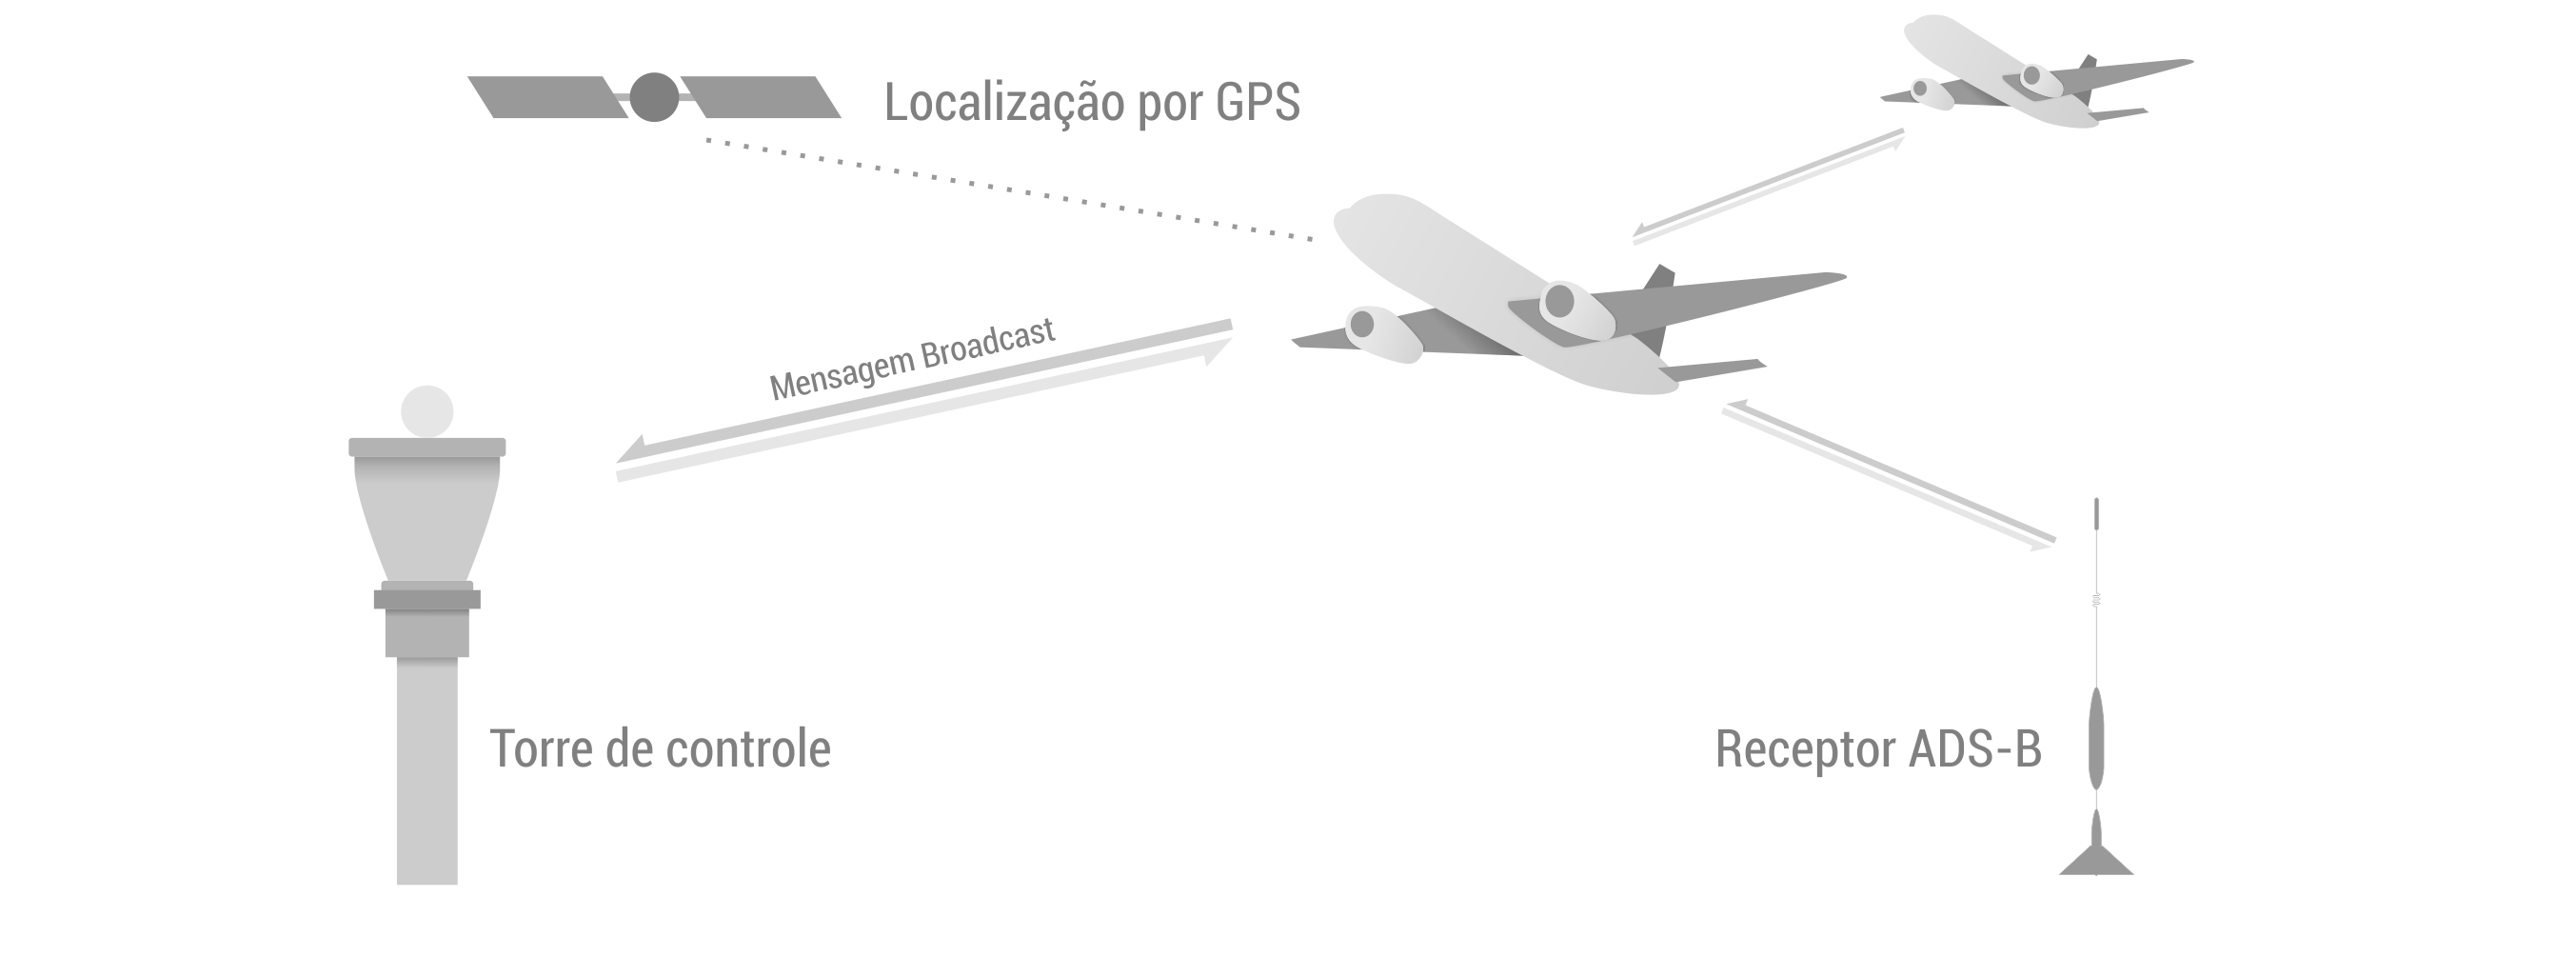
\includegraphics[scale=0.67]{figuras/ads-b} % altere o atributo scale para o tamanho da figura
    }
    
\legend{Fonte: Elaborada pelo autor}
    	
\end{figure}

\subsection{Análise e Detecção de Colisão Entre Aeronaves no Espaço Aéreo}
Com o auxílio de tecnologias modernas de coleta de dados como a ADS-B, é possível monitorar com precisão e rapidez as milhares de aeronaves que sobrevoam o planeta simultaneamente. Mas utilizar tais dados para a análise e detecção de colisão exige algoritmos em sua maioria complexos e com vários problemas de otimização. Um exemplo de algoritmo relativamente simples e eficiente é apresentado no trabalho de \citeonline{Gariel2011}, o qual será utilizado neste trabalho em testes de escalabilidade.

O algoritmo de \citeonline{Gariel2011} considera duas zonas em torno da aeronave que garantem sua segurança. A primeira zona se chama Collision Airspace Zone (CAZ), uma região cilíndrica com 160 metros de raio e 60 metros de altura, cujas dimensões consideram o tamanho das aeronaves atuais e possíveis imprecisões em sua localização. Se outra aeronave cruzar essa zona, estará correndo um risco sério de colisão. A Protection Airspace Zone (PAZ) determina uma região cilíndrica em torno da aeronave, normalmente maior que a região CAZ, que não tem seu foco em prever uma colisão iminente, mas sim proporcionar um voo confortável para o piloto, mantendo-o suficientemente distante de outros voos. Seu tamanho é calculado em função de sua velocidade relativa a uma segunda aeronave. Por tanto, a região PAZ é dinâmica e varia dependendo do par de aeronaves que está sendo verificado. As dimensões da região PAZ podem ser obtidas com:
\[ R_{PAZ}(t) = R_{PAZ, min} + max(0, V_{R}(t))\tau _{hor} \]
\[ H_{PAZ}(t) = H_{PAZ, min} + max(0, V_{R, vert}(t))\tau _{vert} \]
onde \(R_{PAZ, min} = R_{CAZ} = 160\, metros\), \(V_{R}(t)\) é a velocidade horizontal relativa entre as aeronaves no instante \(t\), \(\tau_{hor} = 10s\) é uma constante de tempo para a dimensão horizontal de PAZ, \(H_{PAZ, min} = 91\, metros\) é a altura mínima de PAZ, \(V_{R, vert}(t)\) é a velocidade vertical relativa entre as aeronaves e \(\tau_{ver} = 10s\) é uma constante de tempo para a dimensão vertical de PAZ.

O algoritmo também prevê alertas distintos para cada tipo de conflito. Caso uma aeronave esteja prestes a entrar na região PAZ de outra dentro dos próximos 15 segundos, um alerta é criado, advertindo que os aviões apresentam uma distância crítica entre si. Se o conflito for detectado para os próximos 15 segundos, outra detecção PAZ é esperada antes que o alerta seja criado, evitando que alertas sejam criados quando uma aeronave cruza momentaneamente a rota de outra. Caso o conflito seja previsto para menos de 15 segundos, o alerta e criado imediatamente. O alerta CAZ funciona de forma semelhante, mas tem muito mais gravidade por indicar uma colisão iminente.

Além de verificar posição atual do avião, o algoritmo faz uma simulação da rota que será percorrida pelo mesmo nos próximos 15 segundos, baseando-se em sua posição, velocidade e taxa de giro. O valor de \(t\) varia, por tanto, de \(0\) à \(15\), e são verificados conflitos PAZ e CAZ para cada novo valor de posição gerado em função de \(t\). Na verificação de colisão entre duas aeronaves, suas respectivas rotas serão sincronizadas em relação a \(t\) e propagadas simultaneamente. Assim, caso a primeira aeronave tenha enviado sua última informação de posição no instante \(t = 1446520500\) (\textit{timestamp} do dia 3 de novembro de 2015, às 3 horas) e a segunda tenha enviado duas informações em \(t = 1446520400\) e \(t = 1446520600\), será efetuado um cálculo de interpolação cúbica para a descoberta da posição da segunda aeronave exatamente no instante \(t = 1446520500\). A partir dessa sincronização dos valores de \(t\), será feita a simulação das rotas das duas aeronaves.

\subsection{Análise e Detecção de Colisão em Grande Escala}

Mesmo com tecnologias mais precisas para o monitoramento de aeronaves, garantir um voo seguro ainda é um grande desafio. Em seu módulo de detecção de colisão, o sistema Radar Livre pretende evitar colisões entre aeronaves e entre aeronaves e acidentes geográficos, utilizando as informações coletadas por seus receptores ADS-B. No entanto, se o sistema for alimentado com um grande número de aeronaves, o módulo de detecção de colisão irá lidar com um grande problema de escalabilidade. Segundo o site Flightradar24\footnote{www.flightradar24.com}, onde podemos acompanhar o voo de aeronaves em tempo real, às 9h30min do dia 24 de Maio de 2016 eram registradas pouco mais de 12.500 aeronaves em funcionamento ao redor do mundo. Ressalta-se que as aeronaves identificadas eram apenas aquelas que carregavam um transreceptor ADS-B e estavam no raio de alcance de alguma antena do sistema. Portanto essa quantidade deve estar bem abaixo do número real de aeronaves em pleno voo no momento da verificação. Verificar a possibilidade de colisão em tantas aeronaves de forma rápida e eficiente é o principal desafio do módulo de detecção de colisão do sistema Radar Livre.

O sistema TCAS funciona dentro da aeronave e preocupa-se em evitar colisão apenas com as aeronaves vizinhas, não necessitando de uma grande capacidade de processamento na verificação de poucas aeronaves. O sistema Radar Livre utiliza uma base de dados unificada com informações de todas as aeronaves observadas, o que obriga seu módulo de detecção de colisão a analisar a possibilidade de colisão entre todas as aeronaves registradas pelo sistema. Em um espaço aéreo pequeno cruzado por três aviões A, B e C, por exemplo, para detectar com segurança todas as possíveis colisões seria necessário analisar um possível conflito entre os aviões A e B, entre B e C e entre A e C, totalizando 3 verificações. Em uma espaço aéreo com 12.500 aeronaves, seriam necessárias 78.118.750 verificações. Se considerarmos que para se ter um monitoramento preciso devemos atualizar todas as previsões a cada 2 segundos, e que em média 12.500 aeronaves sobrevoam simultaneamente a qualquer hora, chegaremos a 337.730.000.000 verificações diárias e o problema de escalabilidade fica claro.



\section{PROCEDIMENTOS METODOLÓGICOS}

As etapas seguidas na realização deste trabalho estão listados abaixo.

\subsection{Revisão Bibliográfica}

Antes de mais nada, foram realizadas pesquisas em trabalhos já existentes com foco na compreensão do funcionamento geral dos sistemas de monitoramento aéreo, bem como o conhecimento das novas tecnologias utilizadas. A tecnologia ADS-B recebeu um atenção especial por ser um componente fundamental do sistema Radar Livre. Em seguida, foram analizados trabalhos direcionados à previsão e tratamento de colisão, alguns abordando o sistema TCAS, e outros trazendo algoritmos de previsão de colisão mais modernos. Entre estes, o algoritmo apresentado no trabalho de \citeonline{Gariel2011} foi selecionado como o mais adequado a compor o módulo CAPLAN. As principais ferramentas de pesquisa foram o Google Acadêmico\footnote{Disponível em scholar.google.com.br} e o site da IEEE\footnote{Disponível em www.ieee.org}. As palavras-chave utilizadas na pesquisa são: monitoramento aéreo, detecção de colisão de aeronaves no espaço aéreo, TCAS e tecnologia ADS-B.

\subsection{Levantamento de Requisitos Para o Módulo CAPLAN}

Após as pesquisas iniciais, foi realizado um levantamento de requisitos para o desenvolvimento do módulo de previsão de colisões CAPLAN, no qual foram listadas as funcionalidades exigidas ao módulo, suas restrições de desempenho e precisão, e os recursos já disponíveis no sistema Radar Livre que darão suporte a previsão de colisão. Os requisitos do módulo são os seguintes:

\begin{itemize}

\item O módulo deve ser capaz de prever a iminência de conflito entre duas aeronaves dadas suas posições globais (latitude, longitude e altitude) e velocidade (velocidade norte-sul, velocidade leste-oeste e velocidade vertical).

\item O módulo deve detectar dois tipos de conflitos: o primeiro tipo indica que as aeronaves apresentam uma distância crítica entre si e que o risco e colisão pode surgir a qualquer momento; o segundo tipo indica uma iminência real de colisão para os próximos segundos.

\item Para cada conflito previsto para dentro dos próximos 15 segundos, um alerta deve ser criado imediatamente. Se um conflito for previsto para exatamente 15 segundos depois que o mesmo fora detectado, deve-se esperar uma segunda previsão de conflito para que a primeira seja validada, o que evita a criação de alarmes desnecessários quando uma aeronave cruza momentaneamente a rota de outra. Essas restrições são especificadas no trabalho de \citeonline{Gariel2011}, e foram adotadas neste trabalho. 

\item Um alerta deve informar qual seu tipo, quais aeronaves estão envolvidas no conflito e quanto tempo resta até que o mesmo ocorra.

\item Após sua criação, os alertas devem ser inseridos no banco de dados disponível no servidor do sistema, para que possam ser acessados pelas aplicações e mostrados aos usuários do sistema. 

\item O módulo deve acessar as informações das aeronaves diretamente no banco de dados disponível no servidor do sistema, de forma a obtê-los o mais rapidamente possível.

\item O módulo terá disponível um servidor com 32 Giga Bytes de memória RAM e 24 núcleos de processamento, recursos que podem oscilar sua disponibilidade devido a hospedagem do servidor Web do sistema e outros processos relativos ao sistema operacional.

\end{itemize}


\subsection{Desenvolvimento do módulo CAPLAN}

Devido à centralização de dados, todas as informações do sistema são processadas em um único lugar, o que exige uma grande capacidade de memória e processamento do sistema. O módulo de detecção de colisão CAPLAN deve, portanto, otimizar ao máximo seu tempo de execução e uso de memória. Para resolução do problema de escalabilidade, o presente trabalho apresenta algumas estratégias de otimização para aplicação em grande escala do algoritmo de \citeonline{Gariel2011}, as quais foram implementadas no módulo e estão listadas abaixo:

\begin{itemize}

\item \textbf{Raio Mínimo de Verificação}: Um Raio Mínimo de Verificação consiste em uma distância mínima que duas aeronaves devem apresentar entre si para que o algoritmo de detecção possa ser executado em ambas. A região de segurança PAZ, apresentada no trabalho de \citeonline{Gariel2011} funciona como um raio mínimo de verificação para as aeronaves. No exemplo da Figura \ref{raio minimo}, a aeronave \textit{D} está fora do raio de verificação de \textit{A} e, portanto, o algoritmo de detecção de colisão não analisará \textit{A} em relação a \textit{B}. Assim, esta solução busca evitar a execução do algoritmo em aeronaves demasiadamente distantes, poupando processamento, memória e tempo de execução.

\begin{figure}[H] %use h para forçar que a figura fique abaixo do texto

\caption{\label{fig:exemplo-1} Demonstração da solução Raio Mínimo com Memorização}

    \fbox{
        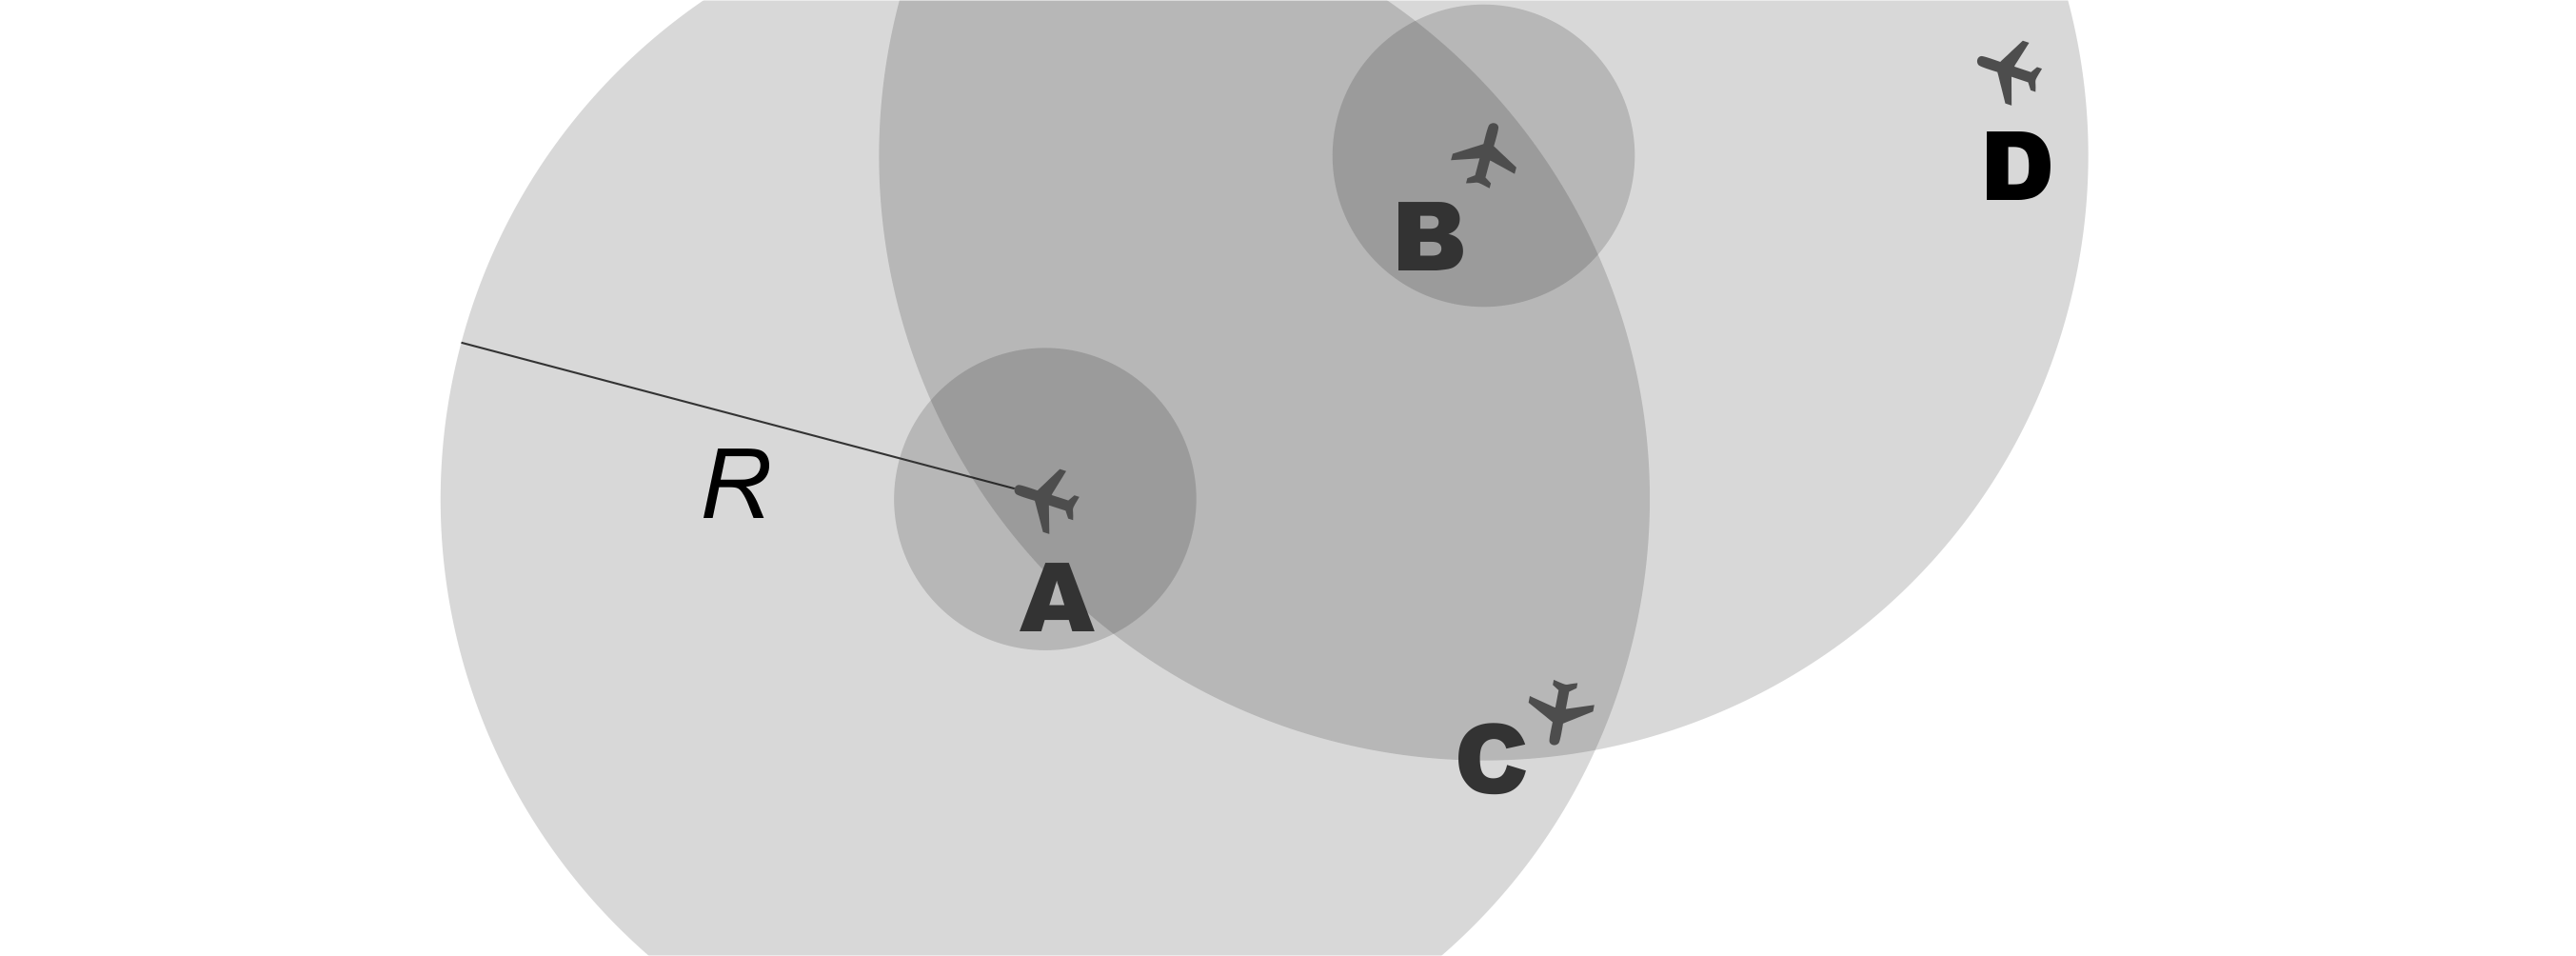
\includegraphics[scale=0.67]{figuras/raio_minimo} % altere o atributo scale para o tamanho da figura
    }
    
\legend{Fonte: Elaborada pelo autor}
\label{raio minimo}
\end{figure}

O próprio algoritmo de detecção de \citeonline{Gariel2011} proporciona o suporte à técnica \textbf{Raio Mínimo de Verificação} com sua região PAZ. Porém, como o algoritmo simula a rota a ser percorrida por cada aeronave nos próximos 15 segundos (intervalo mínimo para o lançamento de alarmes), a região de Raio Mínimo de Verificação será obtida pela região PAZ estendida com a distância que seria percorrida pela aeronave no intervalo de 15 segundos. A não intersecção das regiões de Raio Mínimo de Verificação de duas aeronaves implica que nenhum alarme será lançado agora, e a custosa simulação de rota a ser percorrida pelas aeronaves não será executada. 

\item \textbf{Segunda Estratégia: Multiprocessamento Simétrico}: O multiprocessamento simétrico é uma forma de dividir a execução de um programa entre vários processadores compartilhando a mesma memória. Isso proporciona um aumento linear na eficiência do processamento, proporcional a quantidade de processadores disponíveis. O computador disponível para este experimento tem 24 núcleos de processamento, nos quais os pares de aeronaves podem ser divididos e verificados paralelamente.

O problema de escalabilidade consiste em uma combinação de pares de aeronaves, nos quais o algoritmo de detecção será aplicado. Durante sua execução, o módulo gera uma lista com todos os pares de aeronaves possíveis. Com a técnica de \textbf{Multiprocessamento Simétrico}, a lista de pares é dividida pelo número de processadores disponíveis e a mesma quantidade de \textit{threads} é criada. Cada \textit{thread} executará uma parte da lista independentemente das demais, e os alarmes serão gerados em tempo de execução de forma assíncrona.


\item \textbf{Terceira Estratégia: Divisão do Espaço Aéreo em Áreas}: Assim como a estratégia de \textbf{Raio Mínimo de Verificação}, a \textbf{Divisão do Espaço Aéreo em Áreas} considera que aeronaves muito distante não irão colidir num curto intervalo de tempo e o algoritmo pode simplesmente ignorá-las e analisar somente aeronaves com real chance de colisão a curto prazo. Mas o objetivo agora é dividir o espaço aéreo global em áreas e analisar apenas aeronaves em regiões próximas, evitando analisar aeronaves muito distantes e poupando processamento. 

Existem muitas formas de dividir o globo terrestre em áreas. Estas podem ser representadas, por exemplo, como regiões triangulares que formam um sólido geométrico de 4 faces (tetraedro), 8 faces (octaedro), ou até mesmo 20 faces (icosaedro). Porém, tais representações tridimensionais são computacionalmente complexas, o que as distancia do seu objetivo inicial de proverem uma otimização ao tempo de execução do algoritmo. Uma representação mais simples, a qual é implementada neste experimento, é a divisão do globo terrestre em fatias delimitadas por latitudes específicas. Nesse caso, as aeronaves podem ser classificadas nas fatias com uma simples verificação de sua latitude e apenas aeronaves na mesma fatia ou em fatias vizinhas serão verificadas entre si pelo algoritmo, poupando memória, processamento e tempo de execução.

\end{itemize}

O módulo foi implementado na linguagem de programação C++, devido a sua alta velocidade de execução e flexibilidade no tratamento de memória, sob o paradigma orientado a objetos. As principais classes contias em seu código-fonte são:

\begin{itemize}

\item \textbf{Math}: responsável pelos cálculos vetoriais e geoespaciais presentes no algoritmo de previsão de colisão, incluindo multiplicação, adição, subtração, normalização, rotação e translação de vetores, o cálculo da distância entre dois pontos na superfície da terra com a \textbf{fórmula de haversine} \cite{haversine} e um método de interpolação cúbica com a Spline Catmull-Rom \cite{catmullrom} utilizado na sincronização das rotas das aeronaves durante a execução do algoritmo.

\item \textbf{Combinator}: responsável por formar os pares de aeronaves a serem processados pelo algoritmo e dividi-los em grupos de forma a paralelizar sua execução com a estratégia de \textbf{Multiprocessamento Simétrico}.

\item \textbf{CollisionDetector}: responsável por aplicar o algoritmo de detecção de colisão a cada par de aeronaves, aplicando as estratégias de \textbf{Divisão do Espaço Aéreo em Áreas} e \textbf{Raio Mínimo de Verificação} e gerando os alertas para o sistema.

\item \textbf{Repository}: responsável por carregar as informações das aeronaves. É estendida pela classe \textbf{RealRepository}, que obtém as informações diretamente do banco de dados.

\end{itemize}

Devido à necessidade da realização de testes, o módulo utiliza recursos da linguagem e chamadas de sistema para obter informações sobre consumo de memória e tempo de execução, que são armazenadas em arquivos para posterior análise. Entrementes, a classe \textbf{SinteticRepository} substituiu a classe \textbf{RealRepository} na obtenção de informações de aeronaves. Isso se deve a sua capacidade de disponibilizar dados sintéticos sob as especificações exigidas pelos testes. Se um destes pretende analisar o módulo buscando conflitos em 20.000 aeronaves simultaneamente, por exemplo, a classe \textbf{SinteticRepository} irá sinterizar 20.000 aeronaves, gerando randomicamente suas respectivas latitudes, longitudes, altitudes e velocidades, respeitando intervalos encontrados em dados reais.

Ainda para automação dos testes, foi criado um \textit{scipt} na linguagem de programação Shell, que executa os testes e gera uma planilha com os resultados.



\subsection{Realização da Análise de Desempenho}

Com o módulo em funcionamento e o suporte a testes preparado, as etapas da análise de desempenho tomaram o foco, as quais são listadas a seguir:

\subsubsection{Conhecer o sistema}

O módulo CAPLAN funcionará em uma máquina com 24 núcleos de processamento e 32 Giga Bytes de Memória Ram. Ao seu lado estará funcionando o servidor Web do sistema Radar Livre, que é implementado na linguagem Python em sua versão 2.7.12 e usa o framework DJango\footnote{Mais informações em www.djangoproject.com} em sua versão 1.9. O servidor provê uma API que pode ser usada pelos coletores para envio de novas informações, e por suas aplicações para acesso aos dados registradas pelo sistema. O servidor conta com o Sistema de Gerenciamento de Banco de Dados PostgreSQL\footnote{Mais informações em www.postgresql.org/about}, uma poderosa e robusta ferramenta de código aberto onde estão armazenados todos os dados coletados, e que será acessado pelo módulo.

\subsection{Escolher as Métricas}

As métricas, que constituem restrições a serem respeitadas no experimento, são listadas a seguir:

\begin{itemize}

\item Consumo de memória: a quantidade de memória RAM consumida pelo módulo CAPLAN não deve ultrapassar o limite de 30 Giga Bytes, visto que a quantidade total disponível no servidor é de 32 Giga Bytes e além do módulo, estará em execução o servidor Web do sistema.

\item Tempo de execução: o tempo de execução do algoritmo de detecção de colisão em todas as aeronaves deve ser curto o suficiente para que qualquer alarme seja emitido 15 segundos antes do possível conflito, seja ele PAZ ou CAZ.


\end{itemize}



\subsection{Definir Fatores e Níveis}
Os fatores que podem afetar o experimento e seus respectivos níveis são apresentados a seguir:

\begin{itemize}
    
\item Distribuição em \textit{threads}: a execução do algoritmo será paralelizada em uma quantidade configurável de \textit{threads}. Para este experimento, serão consideradas as quantidades \(n\), \(n-2\) e \(n-4\), onde \(n\) representa o número de núcleos de processamento disponíveis no computador de testes, no caso deste trabalho \(n = 24\). No caso de \(n-2\) e \(n-4\), as quantidades subtraídas são compensações às \textit{threads} utilizadas no restante do módulo de detecção (a \textit{thread main}, a \textit{thread} responsável pela execução da combinação, a \textit{thread} responsável pelo acesso ao banco de dados e a \textit{thread} responsável pelo processamentos dos alarmes gerados). Essa compensação garante que o número de \textit{threads} seja o mesmo que o número de núcleos de processamento. Porém, como algumas partes do módulo exigem mais poder de processamento que outras, não há garantia de que uma mesma quantidade de \textit{threads} e núcleos proporcione um aproveitamento máximo do paralelismo, algo que apenas experimentos podem mostrar.

\item Intervalo de simulação: durante a execução do algoritmo de detecção de colisão, este realiza uma simulação da rota a ser percorrida por cada aeronave em um intervalo configurável de tempo. Este intervalo interfere diretamente no tempo de processamento do algoritmo e a diferença entre os mesmos (intervalo de simulação e tempo de processamento) deve ser de no mínimo 15 segundos, de forma que qualquer alarme seja emitido 15 segundos antes do possível conflito. Os intervalos testados serão de 20, 30, 40, 50 e 60 segundos.

\item Intervalo entre áreas: com a estratégia de divisão em áreas, o globo terrestre é dividido em fatias de intervalo de latitude configurável. Se o intervalo for de 1 grau, por exemplo, as fatias terão altura de um grau de latitude. Para este experimento, serão testados intervalos de 1 a 5 graus.

\end{itemize}


\subsection{Escolher a Técnica de Avaliação}

% ...

\subsection{Executar a Avaliação e Obter os Resultados}

O módulo CAPLAN foi executado várias vezes por um \textit{script} no servidor do sistema Radar Livre. Em sua versão de teste o módulo recebe parâmetros de execução que especificam a quantidade de aeronaves a ser sintetizada, quais técnicas de otimização devem ser utilizadas e quantas vezes o teste deve ser repetido. Os valores utilizados para a quantidade de aeronaves foram 100, 500, 1000, 5000, 10000, 15000, 20000, 25000 e 30000. Para cada um destes valores, foram testadas as possibilidades de execução sem otimizações, com a técnica \textbf{Multiprocessamento Simétrico}, com a técnica \textbf{Divisão em Áreas} e com as duas técnicas simultaneamente. A técnica de \textbf{Raio Mínimo de Verificação} participou de todos os experimentos pois já fazia parte do algoritmo de detecção que é especificada no trabalho de \citeonline{Gariel2011}, onde a região de segurança PAZ representa o raio mínimo. Além disso, cada experimento foi repetido 5 vezes, e os valores finais do tempo de execução e consumo de memória de cada experimento são obtidos pela média aritmética dos valores obtidos pelas repetições dos mesmos.

\subsection{Analisar e interpretar os resultados}
\subsection{Apresentar os Resultados}


\section{Resultados Esperados}

O algoritmo selecionado e uma das duas soluções de escalabilidade farão parte do módulo de detecção de colisão do sistema de monitoramento aéreo Radar Livre. Após a análise de desempenho, poder-se-á calcular precisamente os recursos de hardware e software necessários para a execução do algoritmo sob as duas soluções. Espera-se, que uma destas apresente um consumo de recursos em níveis adequados ao sistema. É necessário, por exemplo, que o consumo de memória RAM seja moderado, pois este é um recurso caro e uma grande necessidade de memória tornaria o sistema inviável. Outra métrica importante a se considerar é o tempo e execução do algoritmo, o qual deve se adequar a um sistema de tempo real. Caso nenhuma das soluções se mostre viável para o sistema, será necessária a formulação de outras que se adequem às métricas exigidas pelo sistema. Este trabalho se propõe a analisar as soluções propostas anteriormente.

% ----------------------------------------------------------
% ELEMENTOS PÓS-TEXTUAIS
% ----------------------------------------------------------
%\postextual

% Referências bibliográficas

\renewcommand{\refname}{REFERÊNCIAS}
\begingroup
\raggedright
\bibliography{bibtex/referencias}
\endgroup
\addcontentsline{toc}{section}{REFERÊNCIAS}
      
% Glossário (Consulte o manual da classe abntex2 para orientações sobre o glossário)
%\glossary

% Apêndices
\apendice{APÊNDICE A}
\addcontentsline{toc}{section}{APÊNDICE A}

Contém materiais de leitura opcional e complementar produzidos pelo autor da pesquisa, incluindo os instrumentos de coleta de dados a serem utilizados. Se não for utilizada, esta seção deve ser removida já na versão 1 do projeto.

% Anexos
% ----------------------------------------------------------
% Anexos
% ---
% Inicia os anexos
% ---

\apendice{ANEXO A}
\addcontentsline{toc}{section}{ANEXO A}

Contém documentos de outros autores, quando aplicável. Se não for utilizada, esta seção deve ser removida já na versão 1 do projeto.

%---------------------------------------------------------------------
% INDICE REMISSIVO
%---------------------------------------------------------------------
%\phantompart
%\printindex
%---------------------------------------------------------------------

\end{document}